\documentclass{standalone}
\usepackage{tikz}
\usetikzlibrary{patterns, positioning}


\begin{document}
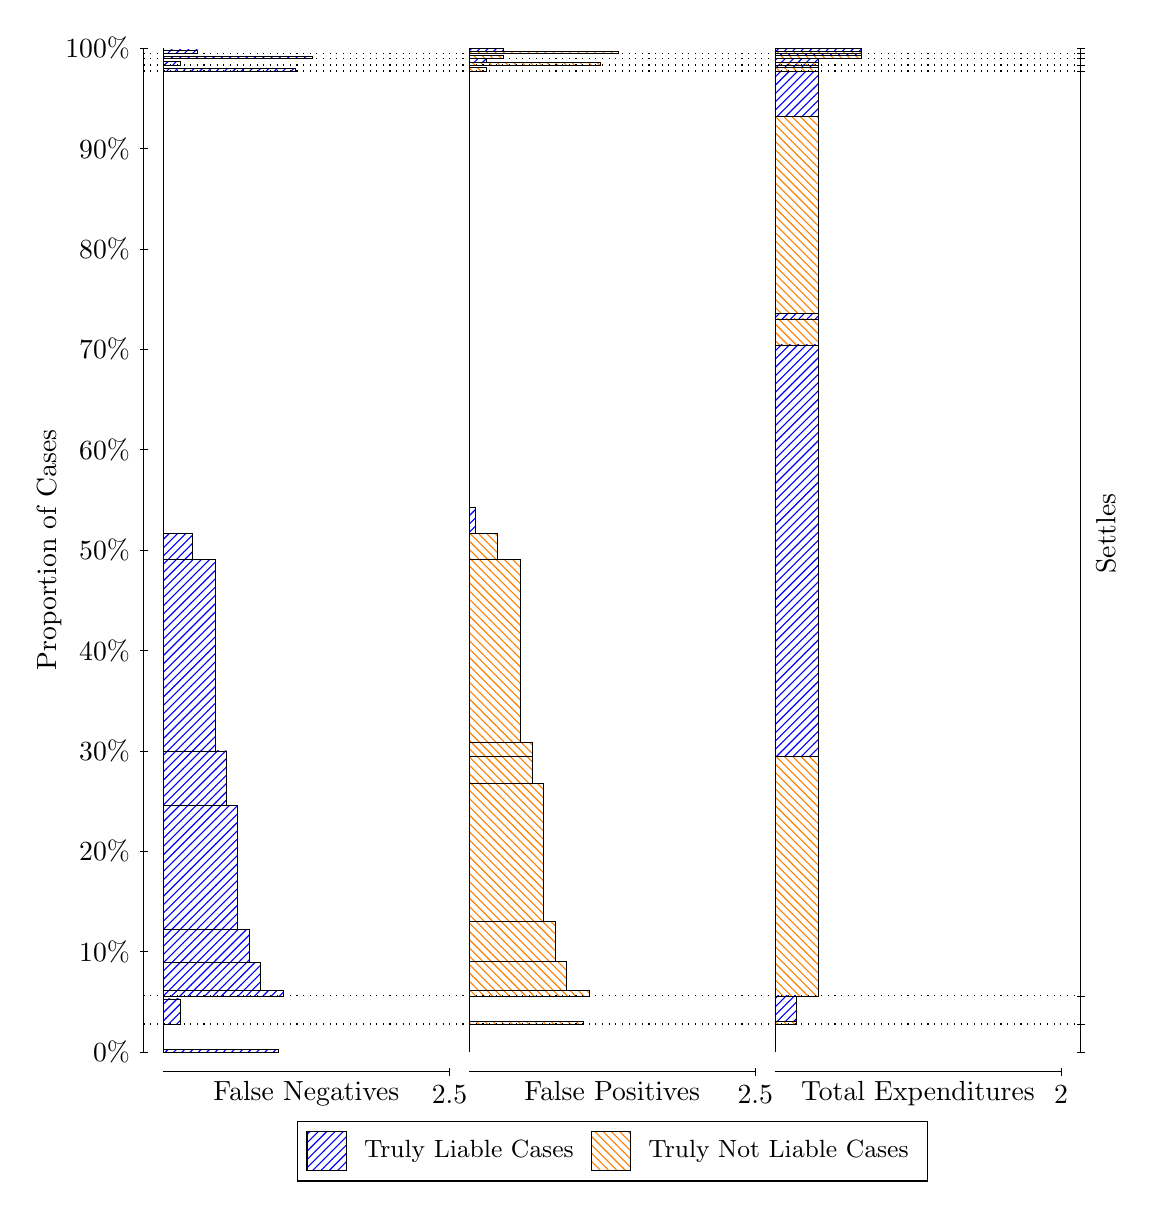
\begin{tikzpicture}
\draw[black, very thin] (1.5,1.75) -- (1.5,14.5);
\node[rotate=90, text=black, anchor=center] at (0.3, 8.125) {Proportion of Cases};
\draw[black, very thin] (1.45,1.75) -- (1.55,1.75);
\node[text=black, anchor=east] at (1.45, 1.75) {0\%};
\draw[black, very thin] (1.45,3.025) -- (1.55,3.025);
\node[text=black, anchor=east] at (1.45, 3.025) {10\%};
\draw[black, very thin] (1.45,4.3) -- (1.55,4.3);
\node[text=black, anchor=east] at (1.45, 4.3) {20\%};
\draw[black, very thin] (1.45,5.575) -- (1.55,5.575);
\node[text=black, anchor=east] at (1.45, 5.575) {30\%};
\draw[black, very thin] (1.45,6.85) -- (1.55,6.85);
\node[text=black, anchor=east] at (1.45, 6.85) {40\%};
\draw[black, very thin] (1.45,8.125) -- (1.55,8.125);
\node[text=black, anchor=east] at (1.45, 8.125) {50\%};
\draw[black, very thin] (1.45,9.4) -- (1.55,9.4);
\node[text=black, anchor=east] at (1.45, 9.4) {60\%};
\draw[black, very thin] (1.45,10.675) -- (1.55,10.675);
\node[text=black, anchor=east] at (1.45, 10.675) {70\%};
\draw[black, very thin] (1.45,11.95) -- (1.55,11.95);
\node[text=black, anchor=east] at (1.45, 11.95) {80\%};
\draw[black, very thin] (1.45,13.225) -- (1.55,13.225);
\node[text=black, anchor=east] at (1.45, 13.225) {90\%};
\draw[black, very thin] (1.45,14.5) -- (1.55,14.5);
\node[text=black, anchor=east] at (1.45, 14.5) {100\%};

\draw[black, very thin] (13.4,1.75) -- (13.4,14.5);
\draw[black, very thin] (13.35,1.75) -- (13.45,1.75);
\node[anchor=west] at (13.35, 1.75) {};
\draw[black, very thin] (13.35,2.1059) -- (13.45,2.1059);
\node[anchor=west] at (13.35, 2.1059) {};
\draw[black, very thin] (13.35,2.4617) -- (13.45,2.4617);
\node[anchor=west] at (13.35, 2.4617) {};
\draw[black, very thin] (13.35,14.208) -- (13.45,14.208);
\node[anchor=west] at (13.35, 14.208) {};
\draw[black, very thin] (13.35,14.285) -- (13.45,14.285);
\node[anchor=west] at (13.35, 14.285) {};
\draw[black, very thin] (13.35,14.366) -- (13.45,14.366);
\node[anchor=west] at (13.35, 14.366) {};
\draw[black, very thin] (13.35,14.433) -- (13.45,14.433);
\node[anchor=west] at (13.35, 14.433) {};
\draw[black, very thin] (13.35,14.5) -- (13.45,14.5);
\node[anchor=west] at (13.35, 14.5) {};

\draw[black, very thin, pattern color=blue, pattern=north east lines] (1.75,1.75) rectangle (3.2033,1.7874);
\draw[black, very thin, pattern color=orange, pattern=north west lines] (1.75,1.7874) rectangle (1.75,2.1059);
\draw[black, very thin, pattern color=blue, pattern=north east lines] (1.75,2.1059) rectangle (1.968,2.4243);
\draw[black, very thin, pattern color=orange, pattern=north west lines] (1.75,2.4243) rectangle (1.75,2.4617);
\draw[black, very thin, pattern color=blue, pattern=north east lines] (1.75,2.4617) rectangle (3.276,2.5345);
\draw[black, very thin, pattern color=blue, pattern=north east lines] (1.75,2.5345) rectangle (2.9853,2.8925);
\draw[black, very thin, pattern color=blue, pattern=north east lines] (1.75,2.8925) rectangle (2.84,3.3034);
\draw[black, very thin, pattern color=blue, pattern=north east lines] (1.75,3.3034) rectangle (2.6947,4.8808);
\draw[black, very thin, pattern color=blue, pattern=north east lines] (1.75,4.8808) rectangle (2.5493,5.5732);
\draw[black, very thin, pattern color=blue, pattern=north east lines] (1.75,5.5732) rectangle (2.404,8.0023);
\draw[black, very thin, pattern color=blue, pattern=north east lines] (1.75,8.0023) rectangle (2.1133,8.3341);
\draw[black, very thin, pattern color=orange, pattern=north west lines] (1.75,8.3341) rectangle (1.75,14.208);
\draw[black, very thin, pattern color=blue, pattern=north east lines] (1.75,14.208) rectangle (3.4213,14.241);
\draw[black, very thin, pattern color=orange, pattern=north west lines] (1.75,14.241) rectangle (1.75,14.285);
\draw[black, very thin, pattern color=blue, pattern=north east lines] (1.75,14.285) rectangle (1.968,14.331);
\draw[black, very thin, pattern color=orange, pattern=north west lines] (1.75,14.331) rectangle (1.75,14.366);
\draw[black, very thin, pattern color=blue, pattern=north east lines] (1.75,14.366) rectangle (3.6393,14.389);
\draw[black, very thin, pattern color=orange, pattern=north west lines] (1.75,14.389) rectangle (1.75,14.433);
\draw[black, very thin, pattern color=blue, pattern=north east lines] (1.75,14.433) rectangle (2.186,14.477);
\draw[black, very thin, pattern color=orange, pattern=north west lines] (1.75,14.477) rectangle (1.75,14.5);
\draw[black, very thin, pattern color=orange, pattern=north west lines] (5.6333,1.75) rectangle (5.6333,2.0684);
\draw[black, very thin, pattern color=blue, pattern=north east lines] (5.6333,2.0684) rectangle (5.6333,2.1059);
\draw[black, very thin, pattern color=orange, pattern=north west lines] (5.6333,2.1059) rectangle (7.0867,2.1433);
\draw[black, very thin, pattern color=blue, pattern=north east lines] (5.6333,2.1433) rectangle (5.6333,2.4617);
\draw[black, very thin, pattern color=orange, pattern=north west lines] (5.6333,2.4617) rectangle (7.1593,2.5345);
\draw[black, very thin, pattern color=orange, pattern=north west lines] (5.6333,2.5345) rectangle (6.8687,2.9031);
\draw[black, very thin, pattern color=orange, pattern=north west lines] (5.6333,2.9031) rectangle (6.7233,3.4119);
\draw[black, very thin, pattern color=orange, pattern=north west lines] (5.6333,3.4119) rectangle (6.578,5.1576);
\draw[black, very thin, pattern color=orange, pattern=north west lines] (5.6333,5.1576) rectangle (6.4327,5.5027);
\draw[black, very thin, pattern color=orange, pattern=north west lines] (5.6333,5.5027) rectangle (6.4327,5.6775);
\draw[black, very thin, pattern color=orange, pattern=north west lines] (5.6333,5.6775) rectangle (6.2873,8.0041);
\draw[black, very thin, pattern color=orange, pattern=north west lines] (5.6333,8.0041) rectangle (5.9967,8.336);
\draw[black, very thin, pattern color=blue, pattern=north east lines] (5.6333,8.336) rectangle (5.706,8.6678);
\draw[black, very thin, pattern color=blue, pattern=north east lines] (5.6333,8.6678) rectangle (5.6333,14.208);
\draw[black, very thin, pattern color=orange, pattern=north west lines] (5.6333,14.208) rectangle (5.8513,14.252);
\draw[black, very thin, pattern color=blue, pattern=north east lines] (5.6333,14.252) rectangle (5.6333,14.285);
\draw[black, very thin, pattern color=orange, pattern=north west lines] (5.6333,14.285) rectangle (7.3047,14.319);
\draw[black, very thin, pattern color=blue, pattern=north east lines] (5.6333,14.319) rectangle (5.8513,14.366);
\draw[black, very thin, pattern color=orange, pattern=north west lines] (5.6333,14.366) rectangle (6.0693,14.41);
\draw[black, very thin, pattern color=blue, pattern=north east lines] (5.6333,14.41) rectangle (5.6333,14.433);
\draw[black, very thin, pattern color=orange, pattern=north west lines] (5.6333,14.433) rectangle (7.5227,14.456);
\draw[black, very thin, pattern color=blue, pattern=north east lines] (5.6333,14.456) rectangle (6.0693,14.5);
\draw[black, very thin, pattern color=orange, pattern=north west lines] (9.5167,1.75) rectangle (9.5167,2.0684);
\draw[black, very thin, pattern color=blue, pattern=north east lines] (9.5167,2.0684) rectangle (9.5167,2.1059);
\draw[black, very thin, pattern color=orange, pattern=north west lines] (9.5167,2.1059) rectangle (9.7892,2.1433);
\draw[black, very thin, pattern color=blue, pattern=north east lines] (9.5167,2.1433) rectangle (9.7892,2.4617);
\draw[black, very thin, pattern color=orange, pattern=north west lines] (9.5167,2.4617) rectangle (10.062,5.5027);
\draw[black, very thin, pattern color=blue, pattern=north east lines] (9.5167,5.5027) rectangle (10.062,10.729);
\draw[black, very thin, pattern color=orange, pattern=north west lines] (9.5167,10.729) rectangle (10.062,11.061);
\draw[black, very thin, pattern color=blue, pattern=north east lines] (9.5167,11.061) rectangle (10.062,11.134);
\draw[black, very thin, pattern color=orange, pattern=north west lines] (9.5167,11.134) rectangle (10.062,13.635);
\draw[black, very thin, pattern color=blue, pattern=north east lines] (9.5167,13.635) rectangle (10.062,14.208);
\draw[black, very thin, pattern color=orange, pattern=north west lines] (9.5167,14.208) rectangle (10.062,14.252);
\draw[black, very thin, pattern color=blue, pattern=north east lines] (9.5167,14.252) rectangle (10.062,14.285);
\draw[black, very thin, pattern color=orange, pattern=north west lines] (9.5167,14.285) rectangle (10.062,14.319);
\draw[black, very thin, pattern color=blue, pattern=north east lines] (9.5167,14.319) rectangle (10.062,14.366);
\draw[black, very thin, pattern color=orange, pattern=north west lines] (9.5167,14.366) rectangle (10.607,14.41);
\draw[black, very thin, pattern color=blue, pattern=north east lines] (9.5167,14.41) rectangle (10.607,14.433);
\draw[black, very thin, pattern color=orange, pattern=north west lines] (9.5167,14.433) rectangle (10.607,14.456);
\draw[black, very thin, pattern color=blue, pattern=north east lines] (9.5167,14.456) rectangle (10.607,14.5);
\draw[black, dotted] (1.5,2.1059) -- (13.4,2.1059);
\draw[black, dotted] (1.5,2.4617) -- (13.4,2.4617);
\draw[black, dotted] (1.5,14.208) -- (13.4,14.208);
\draw[black, dotted] (1.5,14.285) -- (13.4,14.285);
\draw[black, dotted] (1.5,14.366) -- (13.4,14.366);
\draw[black, dotted] (1.5,14.433) -- (13.4,14.433);
\draw[black, very thin] (1.75,1.5) -- (5.3833,1.5);
\node[text=black, anchor=north] at (3.5667, 1.5) {False Negatives};
\draw[black, very thin] (5.3833,1.45) -- (5.3833,1.55);
\node[text=black, anchor=north] at (5.3833, 1.45) {2.5};

\draw[black, very thin] (5.6333,1.5) -- (9.2667,1.5);
\node[text=black, anchor=north] at (7.45, 1.5) {False Positives};
\draw[black, very thin] (9.2667,1.45) -- (9.2667,1.55);
\node[text=black, anchor=north] at (9.2667, 1.45) {2.5};

\draw[black, very thin] (9.5167,1.5) -- (13.15,1.5);
\node[text=black, anchor=north] at (11.333, 1.5) {Total Expenditures};
\draw[black, very thin] (13.15,1.45) -- (13.15,1.55);
\node[text=black, anchor=north] at (13.15, 1.45) {2};



\node[text=black, centered, rotate=90] at (13.72, 8.335) {Settles};





\draw (7.449999999999999,1.5) node[draw=none] (baseCoordinate) {};
\begin{scope}[align=center]
        \matrix[scale=0.5, draw=black, below=0.5cm of baseCoordinate, nodes={draw}, column sep=0.1cm]{
            \node[rectangle, draw, minimum width=0.5cm, minimum height=0.5cm, pattern color=blue, pattern=north east lines] {}; &
            \node[draw=none, font=\small, text=black] (B) {Truly Liable Cases}; &
            \node[rectangle, draw, minimum width=0.5cm, minimum height=0.5cm, pattern color=orange, pattern=north west lines] {}; &
            \node[draw=none, font=\small, text=black] (B) {Truly Not Liable Cases}; \\
            };
\end{scope}

\end{tikzpicture}
\end{document}